\documentclass{article}
\usepackage[a4paper, total={7in, 9in}]{geometry}
\usepackage{graphicx} % Required for inserting images
\usepackage{booktabs}
\usepackage{url}
\usepackage{amsmath}
\usepackage{amsfonts}
\usepackage{placeins}
\usepackage{float}


\title{CROBEX index rebalancing effects}
\author{Albert Maršić, Damjan Crnković, Mihael Vranić \\ 
        Mentor: doc. dr. sc. Stjepan Begušić}
\date{January 2026}

\begin{document}

\maketitle
\begin{abstract}
We study the short-horizon price effects of CROBEX index rebalancing at the Zagreb Stock Exchange. Using all insertions and deletions since 2010, we focus on the period between the official announcement and the effective implementation date. We form equal-weighted event portfolios to compute daily abnormal returns relative to the CROBEX benchmark and calculate cumulative abnormal returns (CAR) around the effective date in a \(\pm 50\) trading-day window. We also evaluate two portfolio constructions: a daily rebalanced event portfolio and a simple announcement-to-effective holding strategy. Average abnormal returns are small and statistically insignificant, while CAR for deletions is persistently negative around implementation. Portfolio evidence shows a strong divergence between insertion and deletion event windows.
\end{abstract}


\section{Introduction}
Stock market indices are key benchmarks for portfolio performance and investment strategies, and changes in their composition can affect stock prices and trading activity. Additions to or removals from an index may lead investors to adjust their portfolios, resulting in abnormal price movements around rebalancing periods.

This paper examines the impact of CROBEX index rebalancing on stock returns at the Zagreb Stock Exchange (ZSE) by analyzing index insertions and deletions since 2010, focusing on stock price behavior in the period between the official rebalancing announcement and the effective insertion or deletion date.

The results contribute to understanding market efficiency and investor behavior, particularly in the context of index-tracking funds and their influence on stock demand on the ZSE.

\section{Related Work}
International evidence on index effects suggests that inclusion and exclusion can trigger short-term price pressure and liquidity shifts, but the magnitude has weakened in recent decades. S\&P Dow Jones Indices document the evolving ``index effect'' in major markets and report that abnormal returns around index changes have attenuated over time \cite{spglobal-index-effect}. The academic literature for large-cap benchmarks reports price and liquidity effects surrounding index membership changes, providing the foundation for event-study analysis \cite{jof-2004-index}.

For the Zagreb Stock Exchange, \v{S}krinjari\'c (2019) analyzes CROBEX composition changes and reports asymmetric reactions in stock returns \cite{skrinjaric2019}. Our study complements this evidence by focusing on the announcement-to-effective window, separating regular and extraordinary updates, and combining abnormal-return tests with portfolio-based performance measures.

\section{Methodology}
\subsection{Data and event construction}
We compile CROBEX rebalancing announcements since 2010 with two key dates per event: the announcement date and the effective inclusion/exclusion date (the first trading day after implementation). Each event is expanded into stock-level records with \texttt{Symbol}, \texttt{AnnDate}, and \texttt{EventDate} and then split into insertions and deletions. Events are also classified as regular or extraordinary rebalancing updates.



Daily price data are taken from a merged dataset where each stock has its own sheet and the benchmark index is stored as \texttt{CBX}. The stock price series were downloaded from the ZSE and consolidated into a single workbook. The regular/extraordinary split required manual cleaning because the ZSE announcements are not consistently formatted for these updates.

Daily returns for the event-window analysis use the \texttt{Change Prev Close Percentage} field, and missing values are filled with zero to avoid dropping days from the aggregated portfolio. All results are based on the available trading days between the announcement and effective dates.

Table~\ref{tab:data_overview} summarizes the sample size and the announcement-to-effective lag (calendar days). Table~\ref{tab:events_by_year} reports the event counts by announcement year with the regular/extraordinary split. Market capitalization and volume are not consistently available in the ZSE downloads, so we do not report those statistics.

\begin{table}[htbp]
\centering
\caption{Sample overview and announcement-to-effective lag (calendar days).}
\label{tab:data_overview}
\begin{tabular}{lrrrrr}
\toprule
Portfolio & Stock-event pairs & Unique events & Unique symbols & Mean lag & Median lag \\
\midrule
Insertions & 101 & 32 & 58 & 13.43 & 12 \\
Deletions & 105 & 41 & 54 & 16.66 & 13 \\
\bottomrule
\end{tabular}
\end{table}

\begin{table}[htbp]
\centering
\caption{Events by announcement year with regular/extraordinary split (stock-event pairs).}
\label{tab:events_by_year}
\scriptsize
\begin{tabular}{rrrrrrr}
\toprule
Year & Ins. & Del. & Reg. Ins. & Extra. Ins. & Reg. Del. & Extra. Del. \\
\midrule
2010 & 3 & 3 & 3 & 0 & 3 & 0 \\
2011 & 7 & 7 & 7 & 0 & 7 & 0 \\
2012 & 5 & 5 & 5 & 0 & 5 & 0 \\
2013 & 4 & 7 & 4 & 0 & 6 & 1 \\
2014 & 10 & 6 & 10 & 0 & 6 & 0 \\
2015 & 16 & 16 & 15 & 1 & 16 & 0 \\
2016 & 6 & 7 & 6 & 0 & 5 & 2 \\
2017 & 6 & 11 & 6 & 0 & 7 & 4 \\
2018 & 5 & 5 & 5 & 0 & 5 & 0 \\
2019 & 1 & 5 & 1 & 0 & 5 & 0 \\
2020 & 11 & 7 & 11 & 0 & 7 & 0 \\
2021 & 5 & 3 & 5 & 0 & 3 & 0 \\
2022 & 7 & 10 & 7 & 0 & 6 & 4 \\
2023 & 7 & 5 & 7 & 0 & 5 & 0 \\
2024 & 4 & 5 & 4 & 0 & 4 & 1 \\
2025 & 4 & 3 & 3 & 1 & 3 & 0 \\
\bottomrule
\end{tabular}
\end{table}

\subsection{Data Cleaning}
\begin{itemize}
\item Parsed announcement and effective dates from ZSE release tables and standardized them.
\item Split insertions/deletions and regular/extraordinary updates; manually corrected labels where ZSE formatting was inconsistent.
\item Normalized tickers (trim whitespace, remove -R-A suffix) to match sheet names.
\item Filled missing daily returns with zero for portfolio aggregation and aligned stock series to the CBX trading calendar.
\item Excluded the DDJH deletion on 2022-07-14 from CAR analysis because of questionable liquidity and reverse stock split following which the company folded.
\end{itemize}

\subsection{Return definitions}
We compute daily returns from prices as \(R_t = (P_t/P_{t-1}) - 1\). The \texttt{Change Prev Close Percentage} column is treated as a decimal return (e.g., 0.0062 corresponds to 0.62\%). Abnormal returns and CAR are reported in percentage points for readability.

\subsection{Event-window abnormal returns}
For each insertion or deletion, we analyze the window from \texttt{AnnDate} to \texttt{EventDate}. On each day, all stocks active in their event windows are combined into an equal-weight portfolio; if $N_t$ stocks are active on day $t$, each contributes $1/N_t$ of its daily return. Abnormal returns are computed as
\[
AR_t = R^{\text{portfolio}}_t - R^{\text{CROBEX}}_t,
\]
where the benchmark return is the CROBEX daily return on the same date. We test the null hypothesis $\mathbb{E}[AR_t]=0$ using a two-sided t-test.

\subsection{CAR around the effective date}
To capture price pressure around implementation, we construct a $\pm 50$ trading-day window around the effective date (day 0). For each event, daily returns are computed from \texttt{Last Price} and abnormal returns are defined as stock return minus CROBEX return. The cumulative abnormal return over a window $[t_1, t_2]$ is
\[
CAR_{[t_1, t_2]} = \sum_{t=t_1}^{t_2} AR_t.
\]
Events are aligned by day offset and averaged across the sample. The DDJH deletion on 2022-07-14 is excluded as an outlier with extreme CAR.

\subsection{Portfolio constructions}
As a complementary view, we construct a daily rebalanced, equal-weight portfolio of all active event-window stocks and compound the aggregate daily return to a portfolio value series. This is done separately for insertions and deletions, and again after splitting events into regular and extraordinary rebalancing groups.

We also evaluate a simple announcement-to-effective event strategy that invests equal capital across all signals on each announcement date and holds each position until the effective date. Proceeds are reinvested as new signals arrive. This portfolio is reported alongside the daily rebalanced approach for comparison. We also evaluate a long–short portfolio that takes long positions in CROBEX additions and short positions in deletions, held from announcement to effective date.


\section{Results}
Table~\ref{tab:data_overview} and Table~\ref{tab:events_by_year} report the sample composition and the regular/extraordinary split by year. Insertions and deletions are of similar size, with slightly more deletion events.

Table~\ref{tab:abnormal_returns} reports the announcement-to-effective abnormal return tests. Average abnormal returns are small in magnitude and not statistically significant at conventional levels for either insertions or deletions.

\begin{table}[htbp]
\centering
\caption{Announcement-to-effective abnormal returns (daily, equal-weighted).}
\label{tab:abnormal_returns}
\begin{tabular}{lrrrrr}
\toprule
Portfolio & $N$ days & Mean AR (\%) & Std.\ dev.\ (\%) & $t$-stat & $p$-value \\
\midrule
Insertions & 309 & 0.21 & 3.10 & 1.20 & 0.232 \\
Deletions & 437 & -0.60 & 7.87 & -1.60 & 0.111 \\
\bottomrule
\end{tabular}
\end{table}


Figure~\ref{fig:r_style_portfolios} shows the daily rebalanced portfolio performance. Over the available sample (2010-01-04 to 2025-10-31), the insertions portfolio grows to 1.56 (cumulative return +56.17\%), while the deletions portfolio declines to 0.0085 (cumulative return -99.15\%).

\begin{figure}[htbp]
\centering
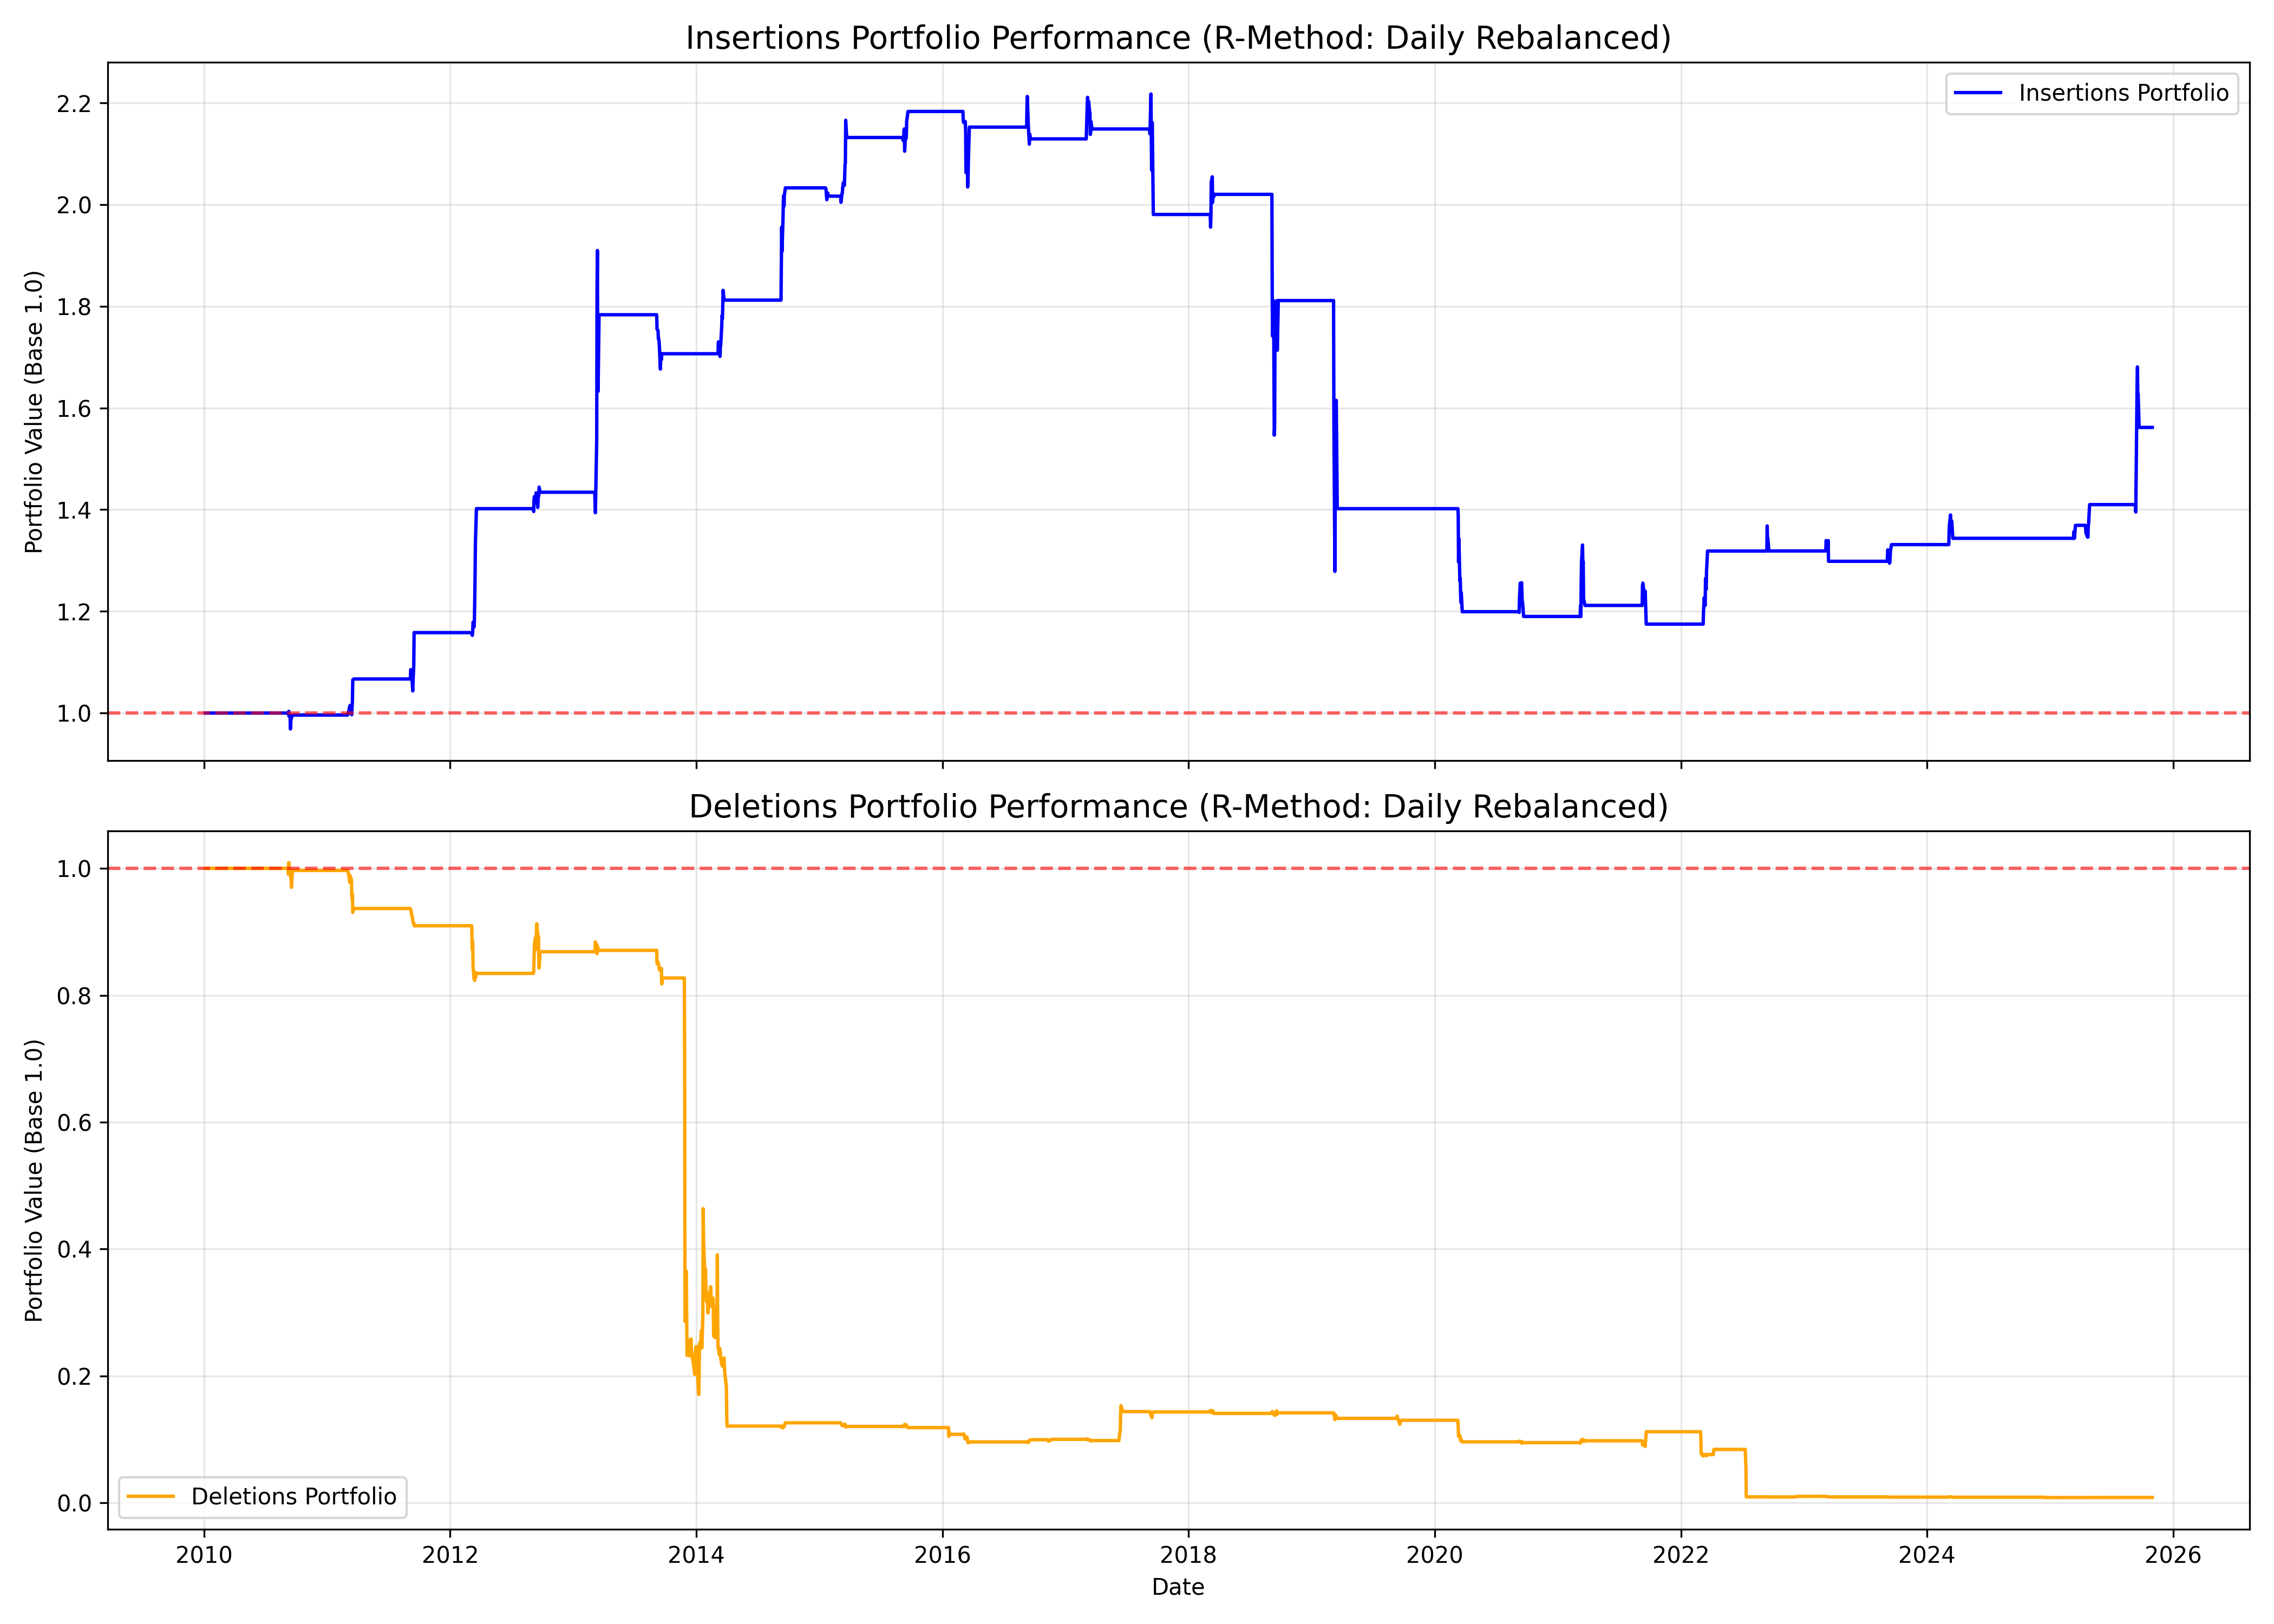
\includegraphics[width=0.95\linewidth]{r_style_analysis_output.png}
\caption{Daily rebalanced portfolios for insertions and deletions (announcement to effective date).}
\label{fig:r_style_portfolios}
\end{figure}

Figure~\ref{fig:r_style_regular_irregular} breaks the rebalanced portfolios into regular and extraordinary events, highlighting that extraordinary deletions dominate the negative tail of the deletions portfolio.

\begin{figure}[htbp]
\centering
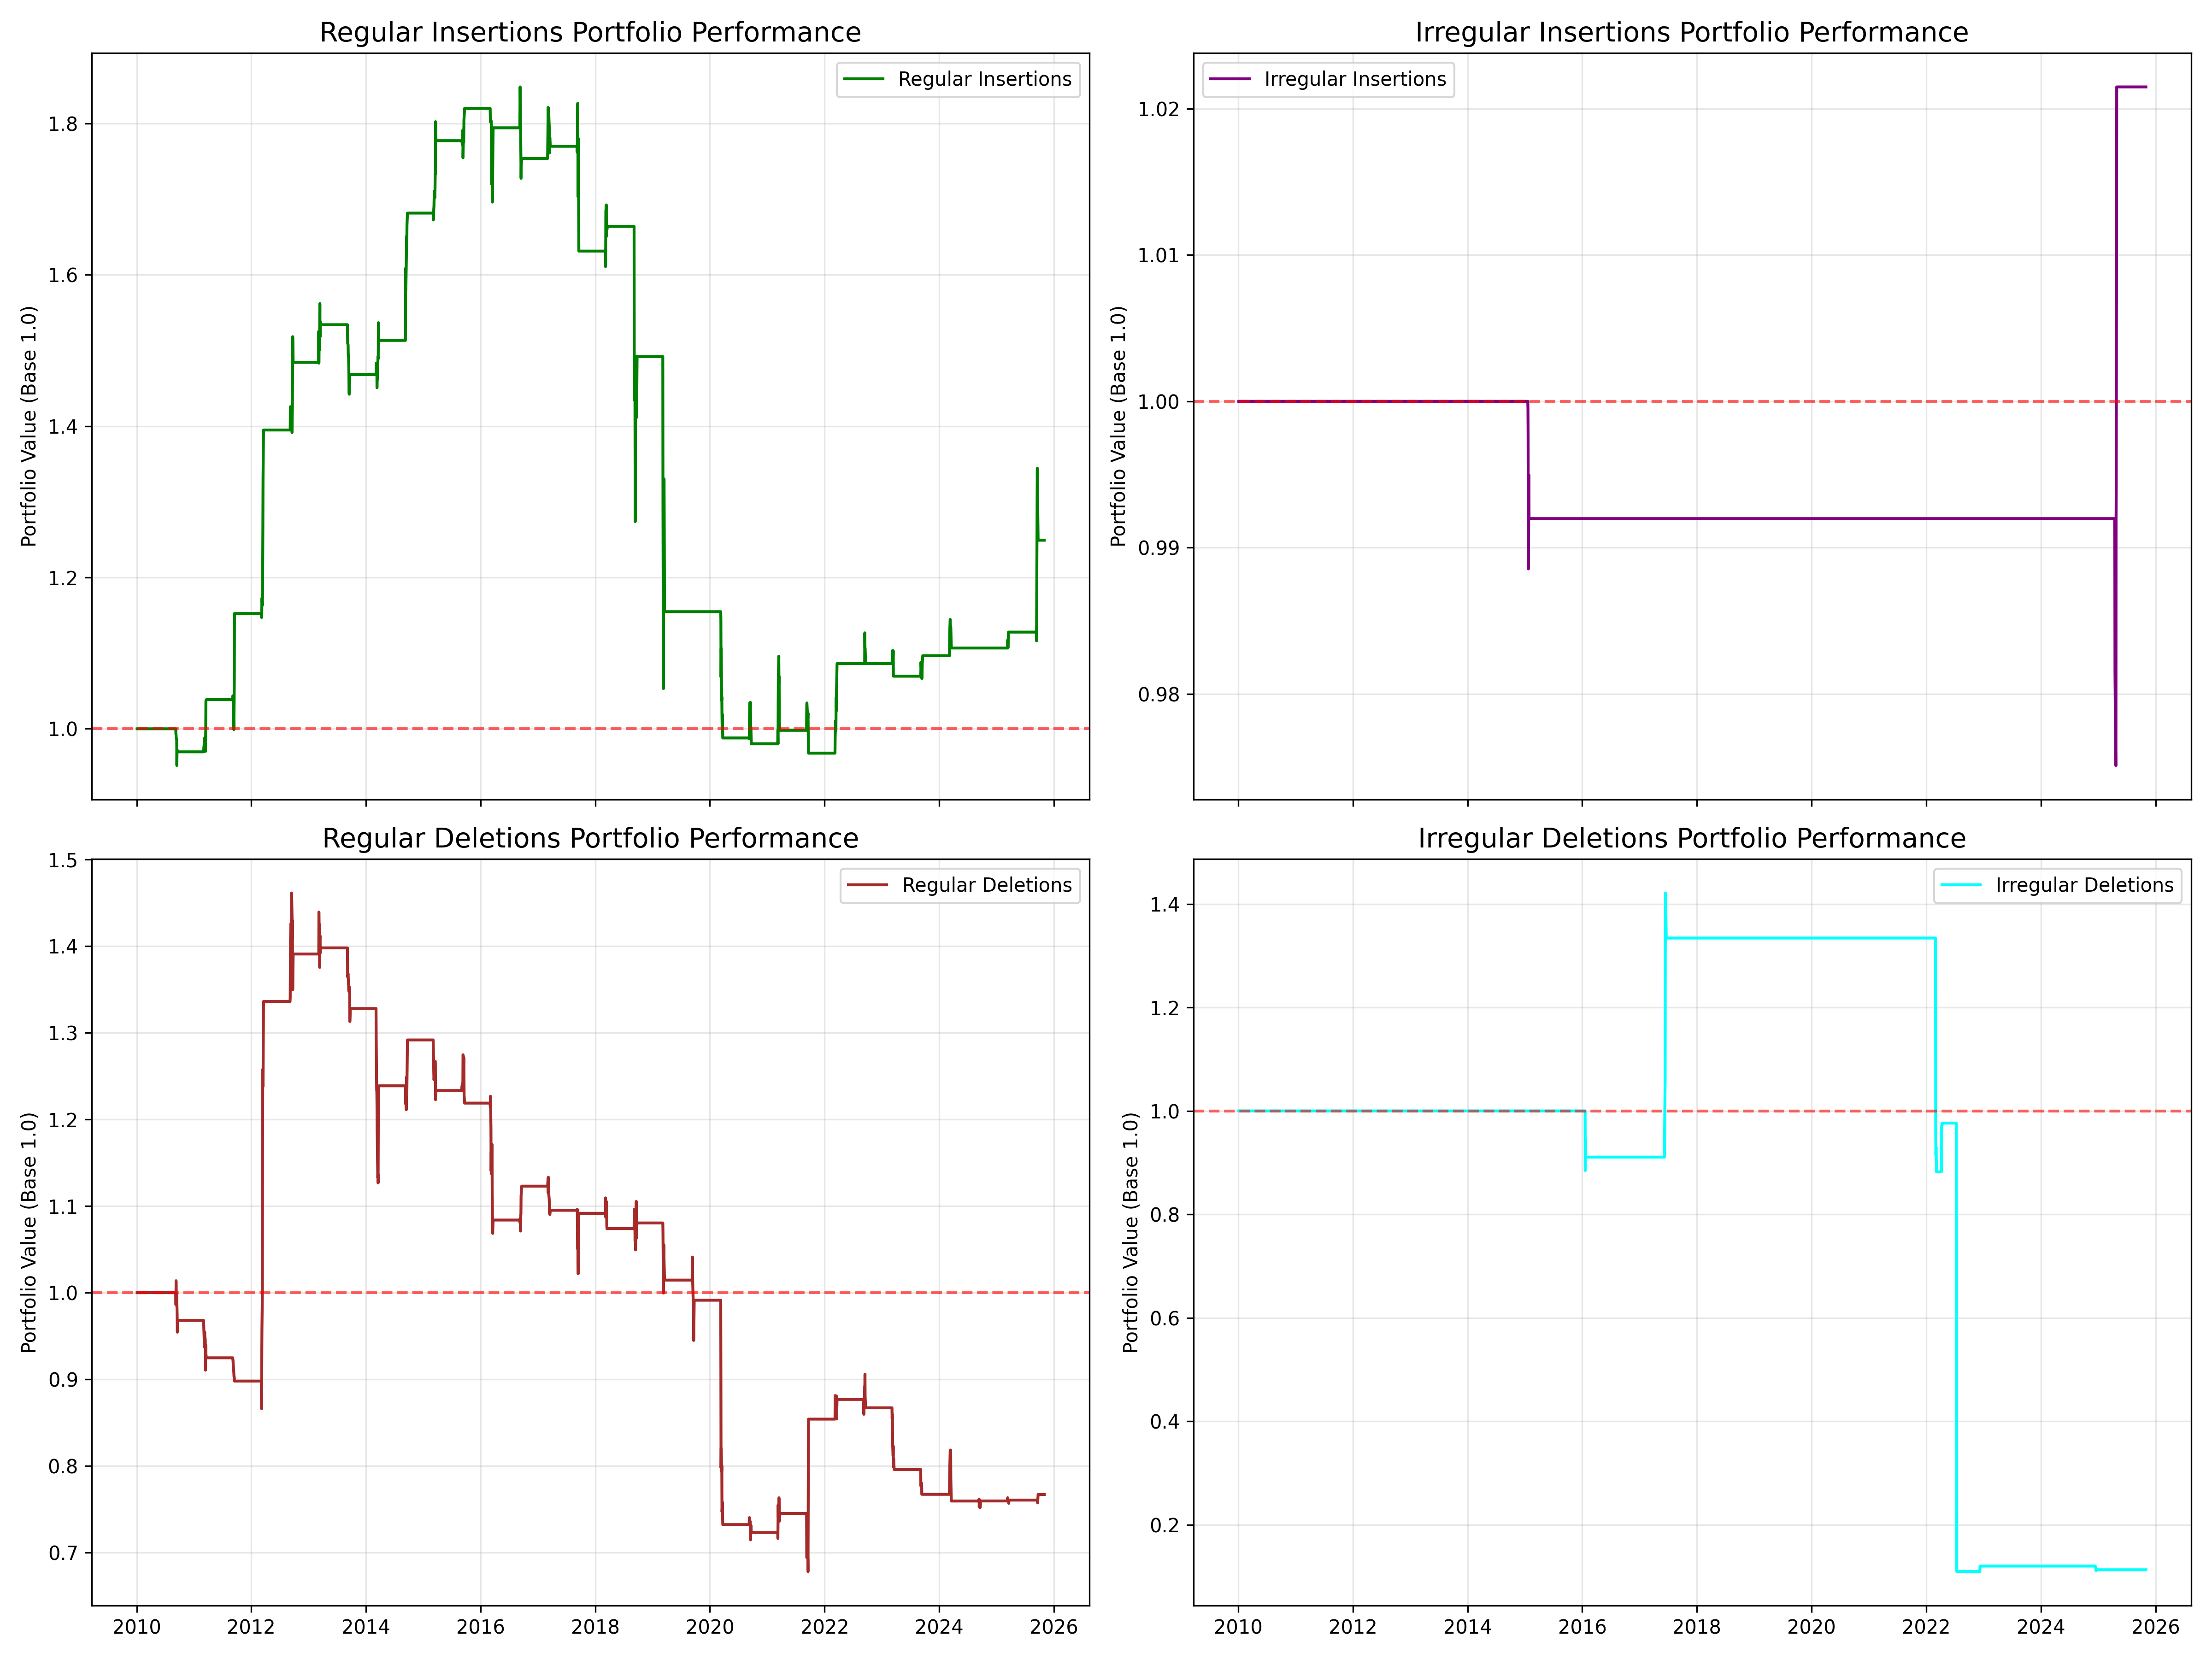
\includegraphics[width=0.95\linewidth]{r_style_detailed_analysis_output.png}
\caption{Daily rebalanced portfolios split by regular vs.\ extraordinary events.}
\label{fig:r_style_regular_irregular}
\end{figure}

Figure~\ref{fig:portfolio_comparison} and Table~\ref{tab:event_portfolio} report the announcement-to-effective event strategy based on equal capital allocation at each announcement date. The insertion portfolio ends at 16,999.80 EUR (+70.00\%), while the deletion portfolio ends at 945.37 EUR (-90.55\%) from an initial 10,000 EUR.

\begin{figure}[htbp]
\centering
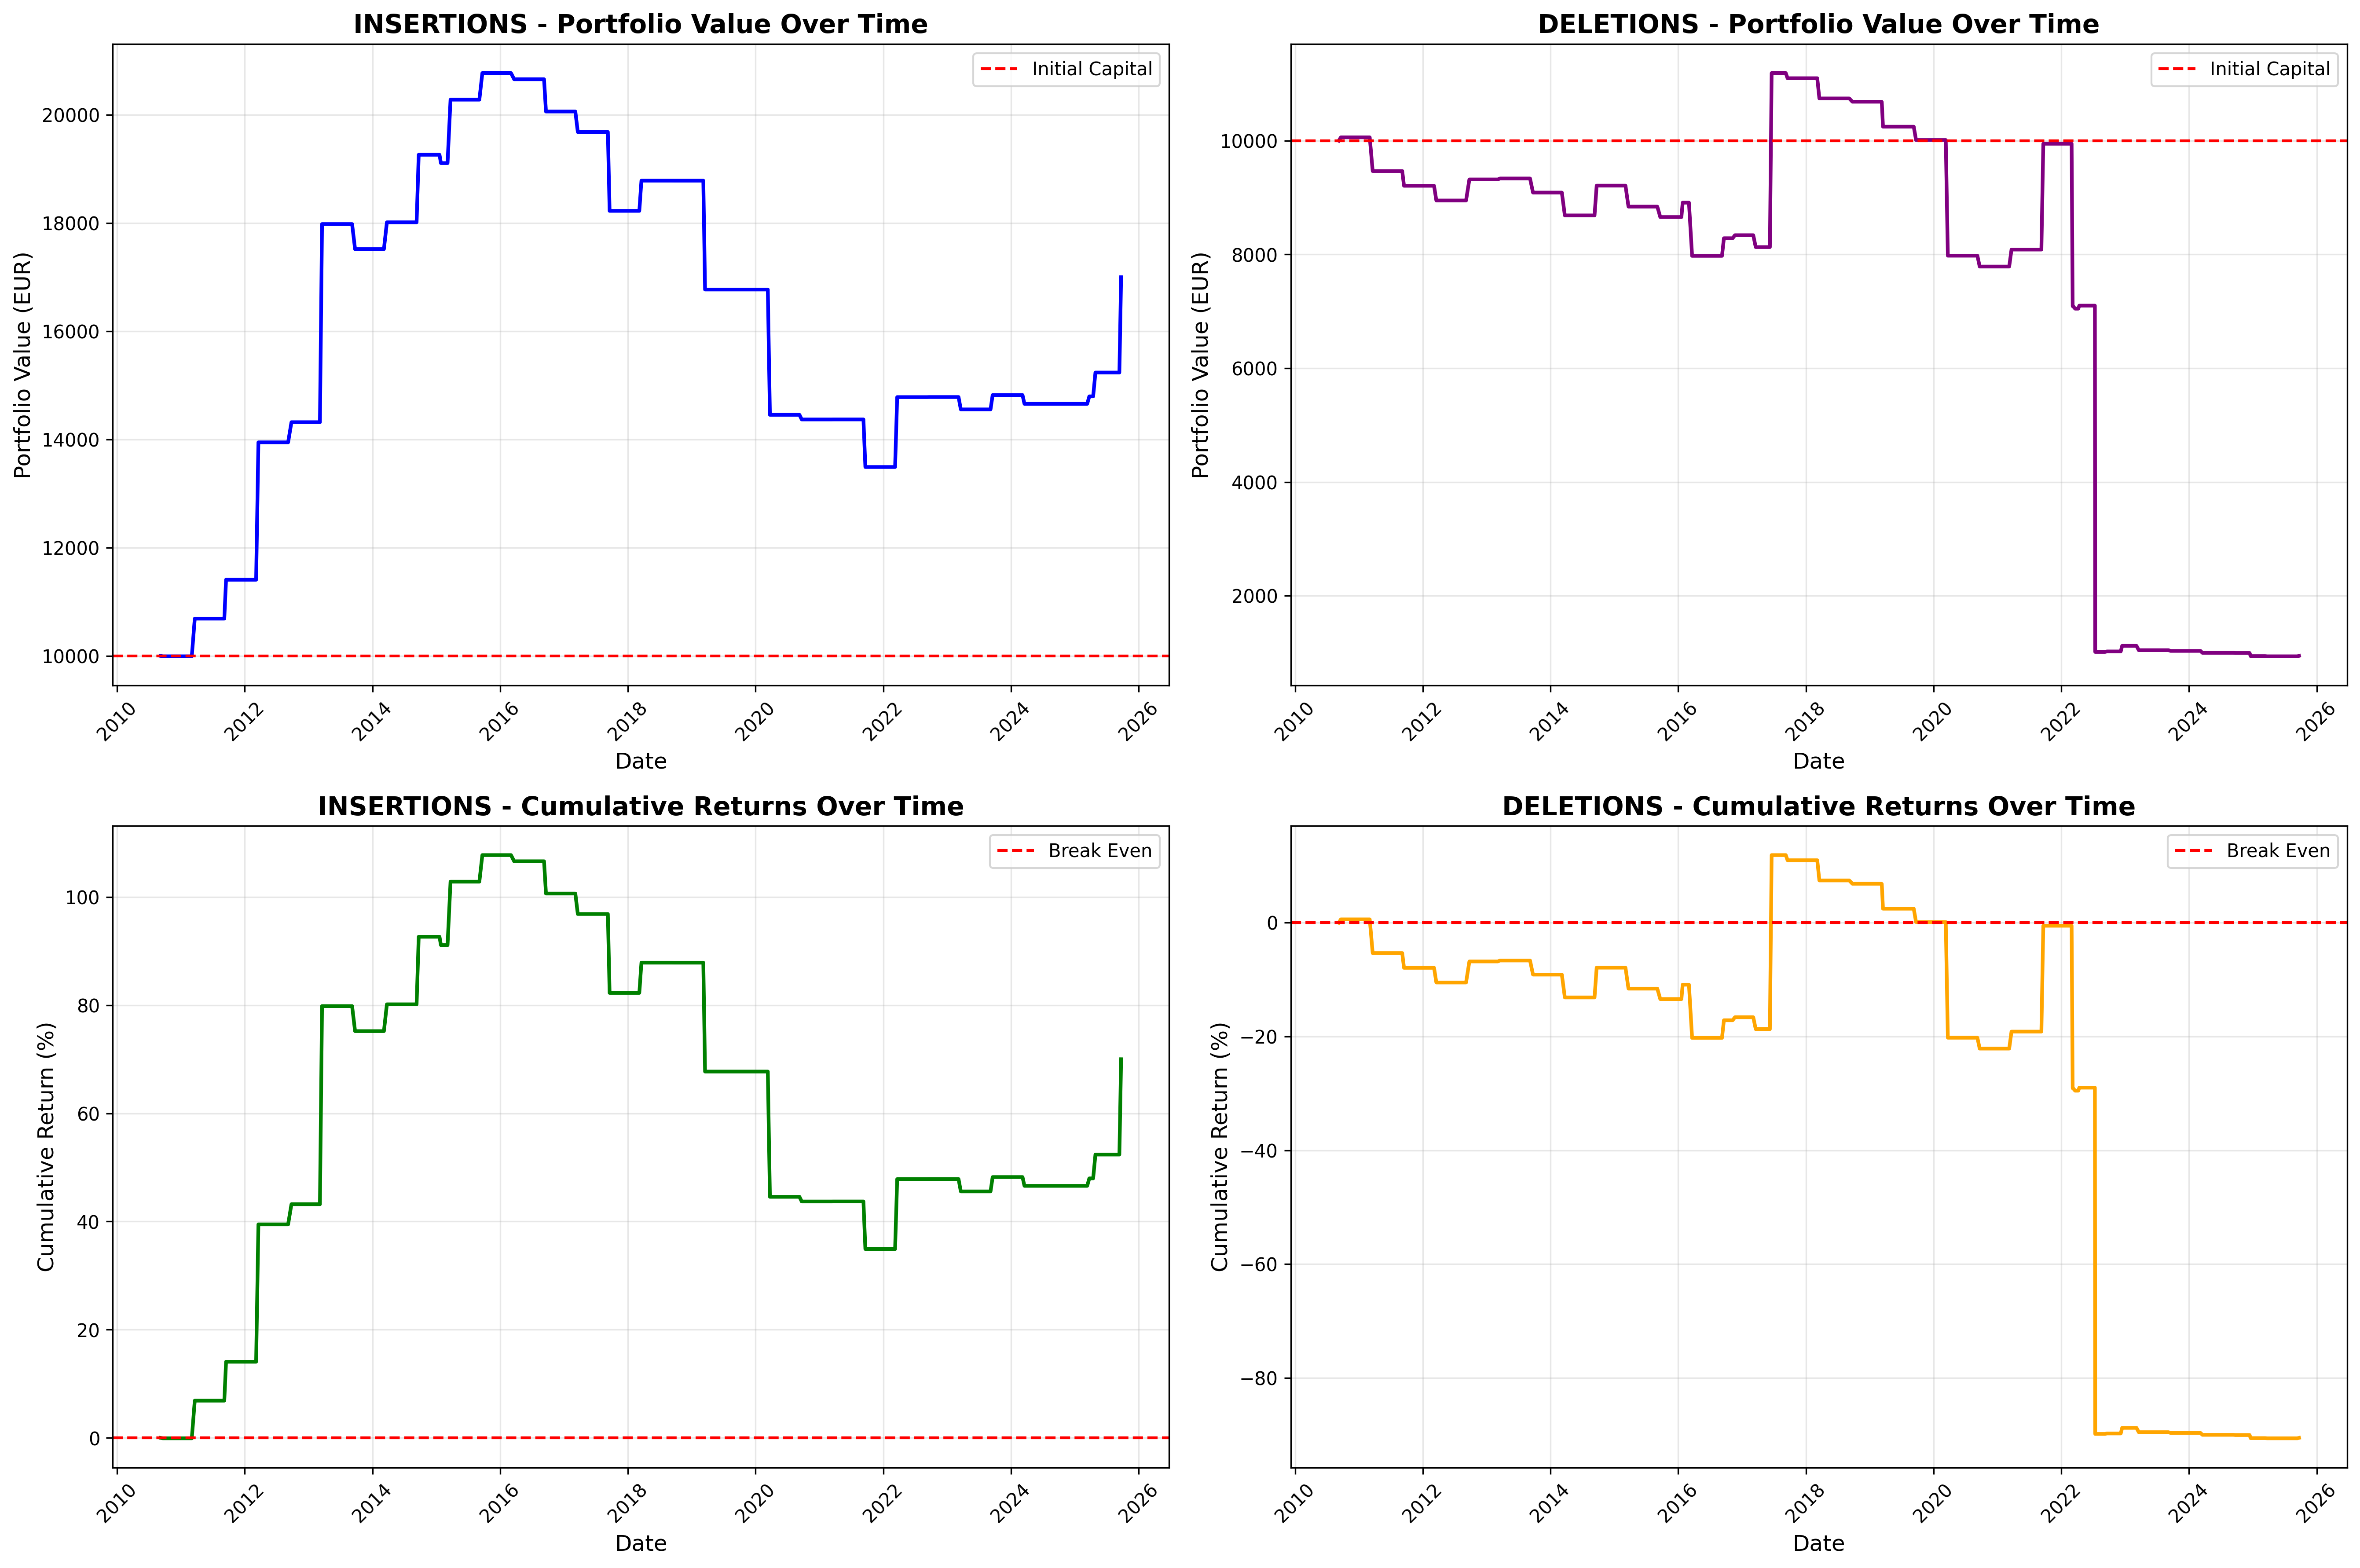
\includegraphics[width=0.95\linewidth]{portfolio_comparison.png}
\caption{Event-trading portfolios (buy at announcement, sell at effective date) with equal capital split per announcement date.}
\label{fig:portfolio_comparison}
\end{figure}

\begin{table}[htbp]
\centering
\caption{Event-trading portfolio performance (initial capital 10,000 EUR).}
\label{tab:event_portfolio}
\begin{tabular}{lrr}
\toprule
Portfolio & Final value (EUR) & Total return (\%) \\
\midrule
Insertions & 16999.80 & 70.00 \\
Deletions & 945.37 & -90.55 \\
\bottomrule
\end{tabular}
\end{table}

Figure~\ref{fig:car_deletions} and Figure~\ref{fig:car_week7_deletions} summarize the average CAR around the effective date for deletions ($n=104$), showing a persistent negative CAR of roughly -5\% before and after the event.

\begin{figure}[htbp]
\centering
\includegraphics[width=0.95\linewidth]{CROBEX-deletions-window50withOutlier.png}
\caption{Average cumulative abnormal return around the effective date for deletions ($\pm 50$ trading days).}
\label{fig:car_deletions}
\end{figure}

\begin{figure}[htbp]
\centering
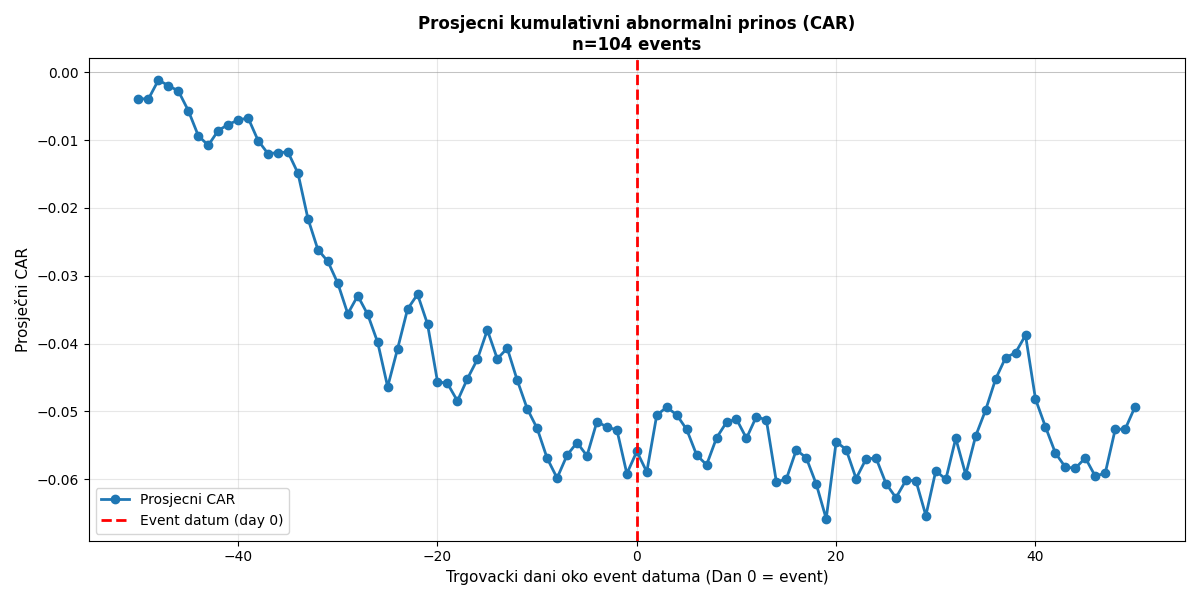
\includegraphics[width=0.95\linewidth]{week7_car_deletions.png}
\caption{Week-7 CAR plot for deletions ($\pm 50$ trading days, DDJH outlier removed).}
\label{fig:car_week7_deletions}
\end{figure}

\begin{figure}[htbp]
\centering
\includegraphics[width=0.95\linewidth]{CAR_insertionsWNDW50.jpeg}
\caption{Average cumulative abnormal return around the effective date for insertions ($\pm 50$ trading days).}
\label{fig:car_insertions}
\end{figure}

\begin{table}[htbp]
\centering
\caption{Average Abnormal Returns (AAR), test statistics and cumulative abnormal returns (CAR) for insertions by day.}
\label{tab:insertions_aar_car_daily}
\begin{tabular}{rrrrr}
\toprule
Day & AAR (\%) & $t$-stat & $p$-value & CAR (\%) \\
\midrule
1  & 0.359  & 0.993  & 0.323 & 0.359 \\
2  & 0.821  & 2.170  & 0.032 & 1.180 \\
3  & 0.023  & 0.077  & 0.939 & 1.204 \\
4  & 0.222  & 0.661  & 0.510 & 1.426 \\
5  & 0.266  & 0.555  & 0.580 & 1.692 \\
6  & -0.038 & -0.151 & 0.881 & 1.654 \\
7  & -0.302 & -0.849 & 0.398 & 1.352 \\
8  & 0.109  & 0.371  & 0.712 & 1.461 \\
9  & 1.164  & 2.790  & 0.007 & 2.625 \\
10 & 0.456  & 0.776  & 0.442 & 3.081 \\
11 & 2.110  & 3.160  & 0.003 & 5.190 \\
12 & -0.300 & -0.589 & 0.560 & 4.890 \\
13 & 2.768  & 2.090  & 0.105 & 7.658 \\
14 & -0.360 & -0.234 & 0.854 & 7.298 \\
\bottomrule
\end{tabular}
\end{table}

\begin{table}[htbp]
\centering
\caption{Average Abnormal Returns (AAR), test statistics and cumulative abnormal returns (CAR) for deletions by day.}
\label{tab:aar_car_deletions}
\begin{tabular}{rrrrr}
\toprule
Day & AAR (\%) & $t$-stat & $p$-value & CAR (\%) \\
\midrule
1  & -1.032 & 2.370 & 0.020 & -1.032 \\
2  & -1.340 & 1.720 & 0.088 & -2.372 \\
3  & -0.909 & 0.985 & 0.327 & -3.280 \\
4  & -0.382 & 1.250 & 0.215 & -3.662 \\
5  & -0.161 & 0.842 & 0.402 & -3.824 \\
6  & 0.035  & -0.098 & 0.922 & -3.789 \\
7  & -0.446 & 1.700 & 0.093 & -4.235 \\
8  & 0.627  & -1.430 & 0.158 & -3.608 \\
9  & 0.086  & -0.220 & 0.826 & -3.522 \\
10 & -0.339 & 0.707 & 0.483 & -3.861 \\
11 & -2.006 & 3.560 & 0.001 & -5.867 \\
12 & 0.328  & -0.573 & 0.571 & -5.540 \\
13 & 0.029  & -0.035 & 0.973 & -5.511 \\
14 & 3.390  & -1.830 & 0.318 & -2.121 \\
\bottomrule
\end{tabular}
\end{table}

\begin{table}[htbp]
\centering
\caption{Cumulative returns for the long–short portfolio scenarios.}
\label{tab:longshort_returns}
\begin{tabular}{lr}
\toprule
Scenario & Cumulative return (\%) \\
\midrule
1 Regular + Extraordinary & +1042.91\% \\
2 Regular only & +100.6\% \\
3 Extraordinary only & +469.75\% \\
\bottomrule
\end{tabular}
\end{table}







\FloatBarrier
\section{Conclusion}
We study CROBEX rebalancing effects using announcement-to-effective windows and find limited evidence of systematic daily abnormal returns for insertions and deletions. CAR around deletion events is persistently negative, suggesting sustained price pressure around implementation. Portfolio evidence reinforces this asymmetry: insertion windows perform strongly, while deletion windows deteriorate sharply in both the daily rebalanced and the event-trading constructions. Future work should incorporate liquidity, volume, and microstructure controls to test whether the observed effects concentrate in thinly traded names.

Limitations include illiquidity in some names, data gaps and zero-imputed returns, event overlap, and the equal-weighting assumption, along with manual cleaning of extraordinary/regular update classifications due to inconsistent ZSE releases. These factors may affect magnitudes but are unlikely to overturn the documented asymmetry between insertions and deletions. The implications are most relevant for small, less liquid markets where index-tracking flows can generate persistent price pressure around implementation.

\appendix

\begin{thebibliography}{9}
\bibitem{spglobal-index-effect}
S\&P Dow Jones Indices.
``What Happened to the Index Effect?''
\url{https://www.spglobal.com/spdji/en/documents/research/research-what-happened-to-the-index-effect.pdf}.

\bibitem{jof-2004-index}
Journal of Finance (2004).
\url{https://onlinelibrary.wiley.com/doi/abs/10.1111/j.1540-6261.2004.00683.x}.

\bibitem{skrinjaric2019}
T. \v{S}krinjari\'c.
``Effects of changes in stock market index composition on stock returns: event study methodology on Zagreb Stock Exchange.''
Croatian Review of Economic, Business and Social Statistics, 5(1), 43--54, 2019.
\end{thebibliography}

\end{document}